\documentclass[tikz,border=12pt]{standalone}
\usepackage[T1]{fontenc}
\usepackage{tgheros}
\usepackage{sfmath}
\usepackage{amsmath}
% % \usepackage{fontawesome5} (Removed for publication-grade academic typography) (Removed for publication-grade academic typography)
\usepackage{tikz}
\usetikzlibrary{arrows.meta,positioning,shapes.geometric,fit,backgrounds,calc}
\usepackage{xcolor}

\renewcommand{\familydefault}{\sfdefault}

% Harvard Crimson & ETH Zurich Academic Semantic Palette
\definecolor{harvardcrimson}{HTML}{A51C30}
\definecolor{ethdarkblue}{HTML}{1F407A}
\definecolor{ethblue}{HTML}{215CAF}
\definecolor{ethpetrol}{HTML}{007A87}
\definecolor{ethbronze}{HTML}{B87333}
\definecolor{ethpurple}{HTML}{5B4B8A}
\definecolor{ethslate}{HTML}{475569}
\definecolor{cardbg}{HTML}{F8FAFC}
\definecolor{cardborder}{HTML}{CBD5E1}
\definecolor{safeTeal}{HTML}{10B981}
\definecolor{alertRed}{HTML}{DC2626}
\definecolor{amberFill}{HTML}{FFFBEB}
\definecolor{amberBorder}{HTML}{F59E0B}

\begin{document}
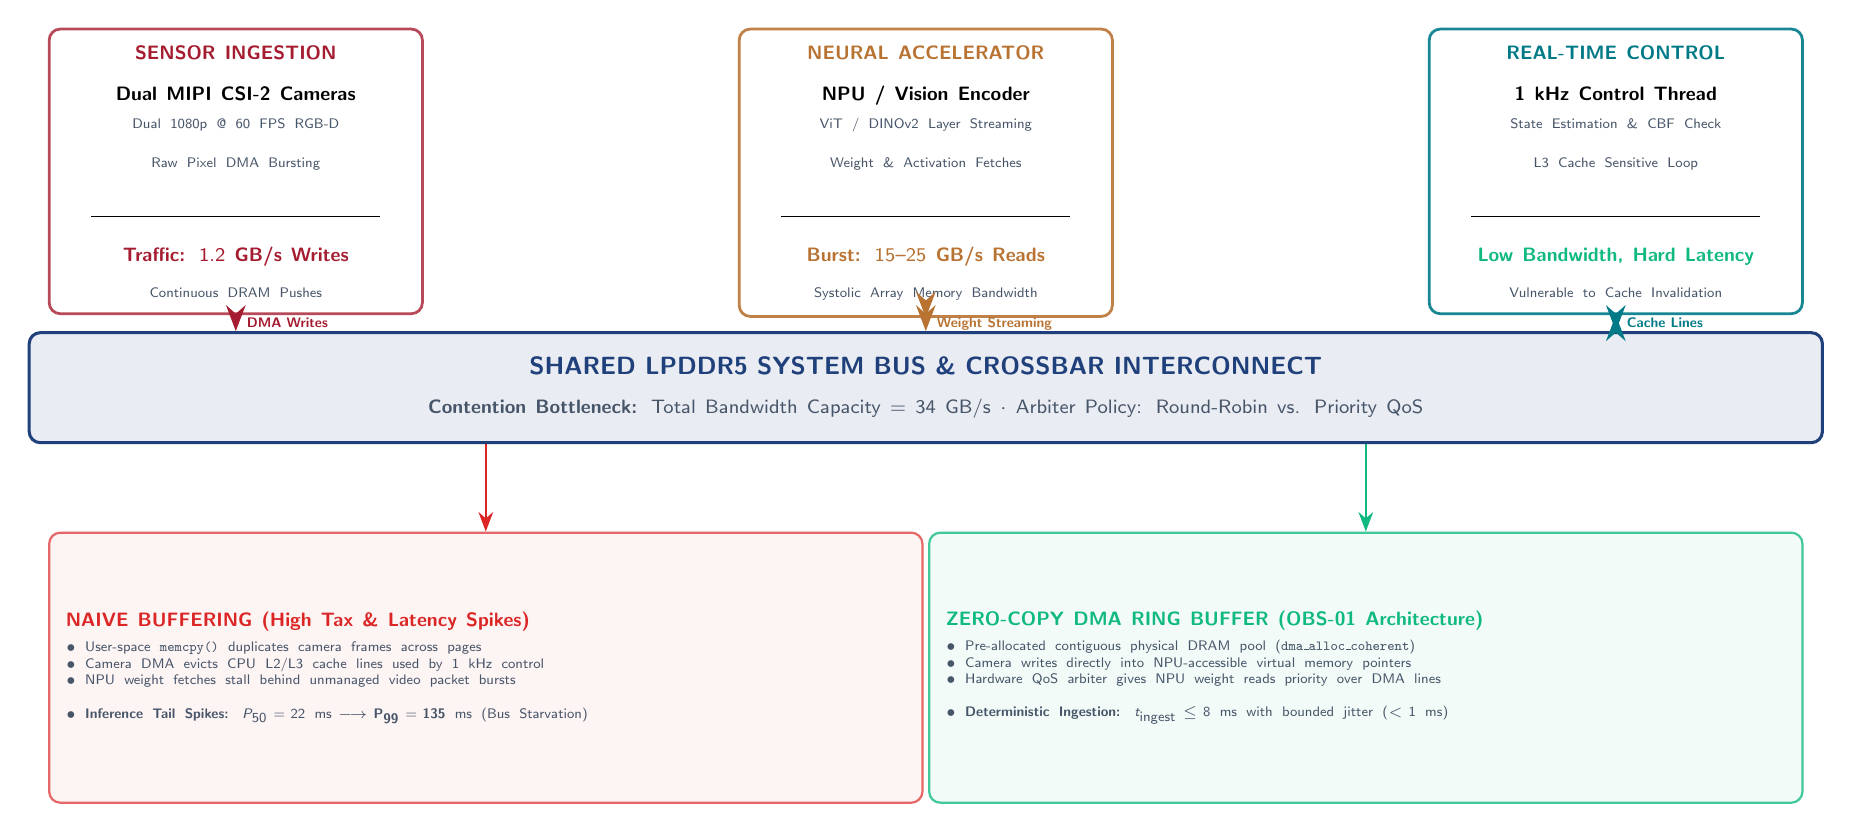
\begin{tikzpicture}[
  font=\sffamily,
  >=Stealth,
  card/.style={
    draw=cardborder,
    fill=cardbg,
    rounded corners=5pt,
    line width=0.9pt,
    inner sep=8pt,
    align=center
  },
  enginebox/.style={
    draw=ethdarkblue,
    fill=white,
    rounded corners=4pt,
    line width=1pt,
    text width=1.70in,
    minimum height=1.35in,
    inner sep=6pt,
    align=center,
    anchor=north
  }
]

  % Top Title Banner
  % (Top title banner removed for academic publication standards)
% Three Subsystems on the SoC
  \node[enginebox, draw=harvardcrimson!80] (cam) at (0.95in, 0.00in) {
    {\scriptsize\bfseries\color{harvardcrimson} SENSOR INGESTION}\\[3pt]
    {\scriptsize\bfseries Dual MIPI CSI-2 Cameras}\\[4pt]
    {\tiny\color{ethslate}Dual 1080p @ 60 FPS RGB-D\\[2pt]Raw Pixel DMA Bursting}\\[6pt]
    \rule{0.85\linewidth}{0.3pt}\\[4pt]
    {\scriptsize\textbf{\color{harvardcrimson}Traffic: $1.2\text{ GB/s}$ Writes}}\\[1pt]
    {\tiny\color{ethslate}Continuous DRAM Pushes}
  };

  \node[enginebox, draw=ethbronze!90] (npu) at (4.40in, 0.00in) {
    {\scriptsize\bfseries\color{ethbronze} NEURAL ACCELERATOR}\\[3pt]
    {\scriptsize\bfseries NPU / Vision Encoder}\\[4pt]
    {\tiny\color{ethslate}ViT / DINOv2 Layer Streaming\\[2pt]Weight \& Activation Fetches}\\[6pt]
    \rule{0.85\linewidth}{0.3pt}\\[4pt]
    {\scriptsize\textbf{\color{ethbronze}Burst: $15\text{--}25\text{ GB/s}$ Reads}}\\[1pt]
    {\tiny\color{ethslate}Systolic Array Memory Bandwidth}
  };

  \node[enginebox, draw=ethpetrol!90] (cpu) at (7.85in, 0.00in) {
    {\scriptsize\bfseries\color{ethpetrol} REAL-TIME CONTROL}\\[3pt]
    {\scriptsize\bfseries 1 kHz Control Thread}\\[4pt]
    {\tiny\color{ethslate}State Estimation \& CBF Check\\[2pt]L3 Cache Sensitive Loop}\\[6pt]
    \rule{0.85\linewidth}{0.3pt}\\[4pt]
    {\scriptsize\textbf{\color{safeTeal}Low Bandwidth, Hard Latency}}\\[1pt]
    {\tiny\color{ethslate}Vulnerable to Cache Invalidation}
  };

  % Shared Interconnect Crossbar & Bus Arbiter
  \node[draw=ethdarkblue, fill=ethdarkblue!10, rounded corners=4pt, line width=1.1pt, text width=8.80in, minimum height=0.55in, inner sep=6pt, align=center] (bus) at (4.40in, -1.80in) {
    {\small\bfseries\color{ethdarkblue} SHARED LPDDR5 SYSTEM BUS \& CROSSBAR INTERCONNECT}\\[2pt]
    {\scriptsize\color{ethslate}\textbf{Contention Bottleneck:} Total Bandwidth Capacity = $34\text{ GB/s}$ $\cdot$ Arbiter Policy: Round-Robin vs. Priority QoS}
  };

  % Arrows into the bus
  \draw[->, line width=1.4pt, draw=harvardcrimson] (cam.south) -- (cam.south |- bus.north)
    node[pos=0.5, right, font=\tiny\bfseries, text=harvardcrimson] {DMA Writes};
  \draw[<->, line width=1.4pt, draw=ethbronze] (npu.south) -- (npu.south |- bus.north)
    node[pos=0.5, right, font=\tiny\bfseries, text=ethbronze] {Weight Streaming};
  \draw[<->, line width=1.4pt, draw=ethpetrol] (cpu.south) -- (cpu.south |- bus.north)
    node[pos=0.5, right, font=\tiny\bfseries, text=ethpetrol] {Cache Lines};

  % Bottom Section: Comparison of Naive Copy vs Zero-Copy Ring Buffer
  \node[draw=alertRed!70, fill=alertRed!5, rounded corners=4pt, line width=0.8pt, text width=4.20in, minimum height=1.35in, inner sep=6pt, align=left] (naive) at (2.20in, -3.20in) {
    {\scriptsize\bfseries\color{alertRed} NAIVE BUFFERING (High Tax \& Latency Spikes)}\\[3pt]
    {\tiny\color{ethslate}
    $\bullet$ User-space \texttt{memcpy()} duplicates camera frames across pages\\
    $\bullet$ Camera DMA evicts CPU L2/L3 cache lines used by 1 kHz control\\
    $\bullet$ NPU weight fetches stall behind unmanaged video packet bursts\\
    $\bullet$ \textbf{Inference Tail Spikes:} $P_{50} = 22\text{ ms} \longrightarrow \mathbf{P_{99} = 135\text{ ms}}$ (Bus Starvation)
    }
  };

  \node[draw=safeTeal!80, fill=safeTeal!5, rounded corners=4pt, line width=0.8pt, text width=4.20in, minimum height=1.35in, inner sep=6pt, align=left] (zerocopy) at (6.60in, -3.20in) {
    {\scriptsize\bfseries\color{safeTeal} ZERO-COPY DMA RING BUFFER (OBS-01 Architecture)}\\[3pt]
    {\tiny\color{ethslate}
    $\bullet$ Pre-allocated contiguous physical DRAM pool (\texttt{dma\_alloc\_coherent})\\
    $\bullet$ Camera writes directly into NPU-accessible virtual memory pointers\\
    $\bullet$ Hardware QoS arbiter gives NPU weight reads priority over DMA lines\\
    $\bullet$ \textbf{Deterministic Ingestion:} $t_{\text{ingest}} \le 8\text{ ms}$ with bounded jitter ($<1\text{ ms}$)
    }
  };

  % Connecting arrows from bus to comparison boxes
  \draw[->, line width=0.9pt, draw=alertRed] (bus.south -| naive.north) -- (naive.north);
  \draw[->, line width=0.9pt, draw=safeTeal] (bus.south -| zerocopy.north) -- (zerocopy.north);

\end{tikzpicture}
\end{document}
